\documentclass[a4paper, 12pt]{article}
\usepackage{amsmath, amssymb}
\usepackage{geometry}  % 控制页面边距
\usepackage{graphicx}  % 插入图片 
\usepackage{hyperref}  % 目录可以跳转
\usepackage{framed}    % 方框 
\geometry{left=2.5cm, right=2.5cm, top=2.5cm, bottom=2.5cm}

\usepackage{fancyhdr}  % 页眉和页脚
\pagestyle{fancy}
\fancyhf{}  % 清除默认设置
\fancyhead[L]{AI Review Notes}  % 左侧页眉内容
\fancyhead[R]{}  % 确保右侧页眉清除
\fancyfoot[C]{\thepage}  % 页脚显示页码

\setlength{\parindent}{0pt} % 取消缩进

% 标题与图片
\title{
    
\includegraphics[width=0.8\textwidth]{Yanami.JPG}\\  % 确保图片路径正确
    AI REVIEW
}
\author{Kinoko}
\date{\today}

\begin{document}

\pagenumbering{gobble}  % 禁用页码

\begin{titlepage}  
    \maketitle
\end{titlepage}

\pagenumbering{roman}  % 使用罗马数字
\fancyhead[R]{}  % 禁用右侧页眉

% 插入目录页
\tableofcontents
\newpage  % 目录单独一页

\pagenumbering{arabic}  % 设置为阿拉伯数字

\section*{Course Syllabus}  % 无编号的章节
\fancyhead[R]{September 22, 2024}  % 手动设置日期
\addcontentsline{toc}{section}{Course Syllabus}  % 手动添加到目录中
    \begin{enumerate}
        \item Introduction to artificial intelligence
        \item Problem solving and search technology
        \item Graph Search Strategies
        \item Evolutionary search
        \item Swarm Intelligence
        \item Memetic algorithms 
        \item Machine learning
        \item Artificial Neural Network
        \item Data mining and knowledge discovery
    \end{enumerate}

\newpage

% 设置章节从 1 开始编号
\setcounter{section}{0}

\section{Introduction}
\fancyhead[R]{September 22, 2024}  % 手动设置日期
    \subsection{What is artificial intelligence?}
        \begin{itemize}
            \item Is an approach to make a computer, a robot, or a product to think \textbf{how smart humans think}.
            \item Artificial Intelligence is a study of how the human brain thinks, learns, decides, and works when it tries to solve problems. And finally, this study outputs intelligent software systems.
            \item Aim of Artificial Intelligence is to improve computer functions which are related to human knowledge, for example, reasoning, learning, and problem-solving.
            \item The objectives of AI research are reasoning, knowledge representation, planning, learning, natural language processing, realization, and the ability to move and manipulate objects. There are long-term goals in the general intelligence sector.
        \end{itemize}
    
    \subsection{Types of AI}
        Artificial Narrow Intelligence(ANI)
        \begin{itemize}
            \item Machine learning
            \item Specialize in one area and solve one problem
        \end{itemize}

        Artificial general Intelligence(AGI)
        \begin{itemize}
            \item Refers to a computer that is as smart as a human across the board
        \end{itemize}

        Artificial Super Intelligence(ASI)
        \begin{itemize}
            \item An intellect that is much smarter than the best human brain in practically any field
        \end{itemize}

    \subsection{Dive into AI understanding}
    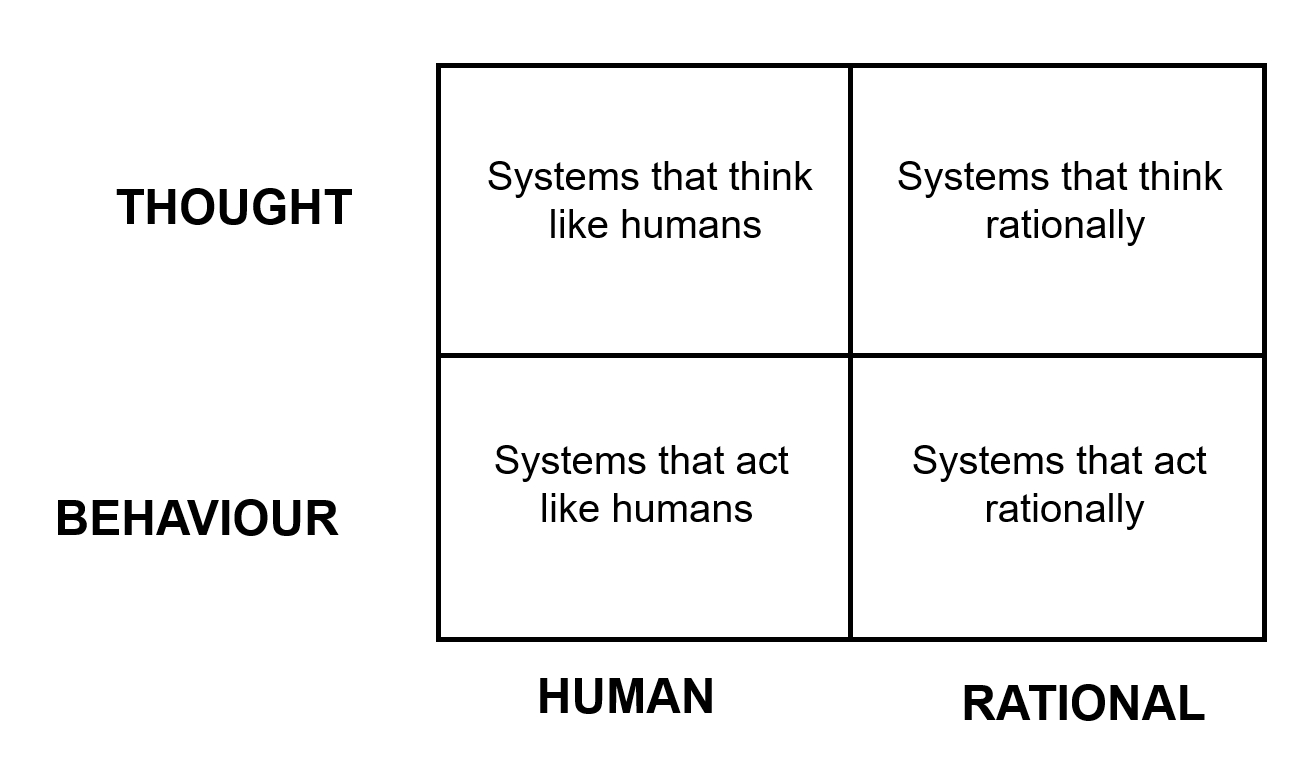
\includegraphics[width=\textwidth]{w1_1.png}

    \section{Problem solving search technology (part1)}
    \subsection{Category of search}
        \subsection*{Incremental Formulation}
        Search algorithm builds a solution step by step, considering only one part of the problem at a time. It incrementally constructs a sequence of decisions or actions to reach the goal.
        \subsection*{Complete-State Formulation}
        The problem and its solution are represented by a complete description of the state of the system or environment. This formulation allows the search algorithm to explore all possible states systematically.
        \subsection*{Toy Problem}
        A simplified, abstract, or small-scale version of a real-world problem. It is often used in AI and search algorithms as a test or learning tool to develop and test algorithms before applying them to more complex problems.
        \subsection*{Real World Problem}
        A complex, practical issue that occurs in real-life scenarios. These problems often involve uncertainty, incomplete information, and multiple interacting factors.
    \subsection{Goodness search of Strategies}
    \begin{itemize}
        \item Completeness
        \item Time complexity
        \item Space complexity
        \item Optimality of the solution (such as path cost)
    \end{itemize}

    \newpage
    \fancyhead[R]{September 25, 2024}

    \subsection{\textbf{Formulate search (Focus!)}}
        \begin{itemize}
            \item States
                \begin{itemize}
                    \item The basic unit for searching.
                    \item Example: Any arrangement of queens on the board is a state. (legal/illegal)
                \end{itemize}
            \item Initial State
                \begin{itemize}
                    \item The state that the agent starts in.
                    \item Example: No queens on the board.
                \end{itemize}
            \item Actions
                \begin{itemize}
                    \item The operations that you can perform for the current state.
                    \item Example: Add a new queen to the board.
                \end{itemize}
            \item Transition Model
                \begin{itemize}
                    \item The outcome of actions.
                    \item Example: Returns the board with a queen added to the specified square.
                \end{itemize} 
            \item Goal test
                \begin{itemize}
                    \item Which determines whether a state is a goal state.
                    \item Example: N queens are all on the board, none attacked happens.
                \end{itemize} 
            \item Path cost
                \begin{itemize}
                    \item Assign a numeric cost to each path.
                    \item Example: Attacked path will cost infinite, otherwise will cost 1.
                \end{itemize} 
        \end{itemize}    

    \subsection{Problem Solving Agent}
        \begin{framed}
            \noindent
            \textbf{function} \textsc{Simple-Problem-Solving-Agent}(\textit{percept}) \textbf{returns} an action \\
            \textbf{static:} \\
            \quad $seq$, an action sequence, initially empty \\
            \quad $state$, some description of the current world state \\
            \quad $goal$, a goal, initially null \\
            \quad $problem$, a problem formulation \\
            
            \noindent
            \textbf{state} $\leftarrow$ \textsc{Update-State}($state$, $percept$) \\
            \textbf{if} $seq$ is empty \textbf{then do} \\
            \quad \textbf{goal} $\leftarrow$ \textsc{Formulate-Goal}($state$) \\
            \quad \textbf{problem} $\leftarrow$ \textsc{Formulate-Problem}($state$, $goal$) \\
            \quad $seq \leftarrow$ \textsc{Search}($problem$) \\
            \textbf{action} $\leftarrow$ \textsc{First}($seq$) \\
            $seq \leftarrow$ \textsc{Rest}($seq$) \\
            
            \noindent
            \textbf{return} $action$
        \end{framed}
    
\newpage
\section{Week 2}
\fancyhead[R]{September 25, 2024}  % 手动设置日期
    \subsection{placeholder}

\end{document}
